\documentclass{article}
\usepackage{algorithm}
\usepackage{algpseudocode}
\usepackage{amsmath}
\usepackage{amssymb}
\usepackage{amsthm}
\usepackage[titletoc]{appendix}
\usepackage{array}
\usepackage[english]{babel}
\usepackage{booktabs}
\usepackage{cancel}
\usepackage{color}
\usepackage{eqparbox}
\usepackage{float}
\usepackage[margin=1in]{geometry}
\usepackage{graphicx}
\usepackage[hidelinks]{hyperref}
% *must* be loaded after hyperref
\usepackage[toc, acronym, numberedsection=nameref]{glossaries}
\usepackage[utf8]{inputenc}
\usepackage{lipsum}
\usepackage{mathtools}
\usepackage[cache=false]{minted}
\usepackage{parskip}
\usepackage{pgfplots}
\usepackage{scalerel}
\usepackage{skull}
\usepackage{subcaption}
\usepackage{titling}
\usepackage{textcomp}
\usepackage{tikz}
\usepackage[compact, explicit]{titlesec}
\usepackage{textcomp}
\usepackage[nottoc]{tocbibind}
\usepackage[textsize=small]{todonotes}
\usepackage[normalem]{ulem}

% Document Settings

\definecolor{__minted_background_color}{rgb}{0.95, 0.95, 0.98}
\definecolor{__minted_highlight_color}{rgb}{0.88, 0.88, 1.0}
\setminted{autogobble=true,
           style=tango,
           breaklines,
           bgcolor=__minted_background_color,
           highlightcolor=__minted_highlight_color,
           mathescape, % Escape math mode everywhere.
           texcomments,  % Enable latex code inside of comments. Useful for referencing equations.
    }

\usetikzlibrary{arrows, automata, shapes, positioning}
\pgfplotsset{compat=1.16}
\numberwithin{equation}{section}
% Sets the width of the margin TODO notes
\setlength{\marginparwidth}{0.84in}
\reversemarginpar{}

% hex #184c9a
\definecolor{__glossary_entry_color}{rgb}{0.094, 0.298, 0.604}
\renewcommand{\glstextformat}[1]{\textbf{\textcolor{__glossary_entry_color}{#1}}}

% Add glos: to the beginning of the glossary labels.
\renewcommand*{\glsautoprefix}{glos:}

% All I want is to have comment italicized, but I cant figure out how
% to properly modify the existing \Comment macro.
% \algrenewcomment[1]{\hfill\eqparbox{COMMENT}{\textit{// #1}}}
\algnewcommand{\IComment}[1]{\Comment{\textit{#1}}}

% TODO: Should this path be relative to the document root or this file?
\graphicspath{{./figures/}}

% Document Definitions

\newcommand{\C}{\mathbb{C}}
\newcommand{\R}{\mathbb{R}}
\newcommand{\Z}{\mathbb{Z}}
\newcommand{\N}{\mathbb{N}}
\renewcommand{\O}{\mathcal{O}}

\theoremstyle{definition}
\newtheorem{defn}{Definition}[section]

\theoremstyle{plain}
\newtheorem{thm}{Theorem}[section]

\renewcommand{\qedsymbol}{$\skull$}

% An inline TODO command. Doesn't play nicely with \todotableofcontents
\newcommand\todoinline[2][]{\todo[inline, caption={TODO}, #1]{
\begin{minipage}{\textwidth-4pt}#2\end{minipage}}}

% Draw clouds around things. Useful in mathematical proofs.
\newcommand{\cloud}[4][\dots]{%
    \raisebox{-0.4\height}{%
        \begin{tikzpicture}
            \node [cloud,
                   draw,
                   cloud puffs=#2,
                   cloud ignores aspect,
                   minimum height=#3,
                   minimum width=#4] {#1};
        \end{tikzpicture}
    }
}

% Use \ceil*{} or \floor*{}
\DeclarePairedDelimiter{\ceil}{\lceil}{\rceil}
\DeclarePairedDelimiter{\floor}{\lfloor}{\rfloor}

\AtBeginDocument{%
\renewcommand{\sectionautorefname}{Problem}
}

% make each \section a problem.
\titleformat{\section}[runin]{\large\bfseries}{}{0pt}{\titlerule[1.5pt]\newline\vspace*{-4pt}
Problem\quad\thesection\newline}[\vspace{0.01ex}{\titlerule[1.5pt]}]


\title{Homework 1}
\author{Austin Gill}
\date{January 25, 2019}

\begin{document}
\maketitle

\section{}
\begin{quote}
    Consider the two sets $S$ and $T$. What relation must hold between the
    two sets such that
    \[\vert S \cup T \vert = \vert S \vert + \vert T \vert \]
\end{quote}

\section{}
\begin{quote}
    Show that $S_1 \cup S_2 = \overline{\overline{S_1} \cap \overline{S_2}}$
\end{quote}

\section{}
\begin{quote}
    Assume we define the \textit{Fibonacci numbers} as $F_0 = 0$, $F_1 = 1$,
    and $F_n = F_{n-1} + F_{n-2}$ for $n \geq 2$. Use mathematical induction to
    prove the following statement for all $n \in \N$.
    \[F_0 + F_1 + \cdots + F_n = F_{n + 2} - 1\]
\end{quote}

\section{}
\begin{quote}
    Find two finite sets $A$ and $B$ such that $A \in B$ and $A \subset B$.
\end{quote}

This is a much simpler problem than it first seemed. First pick $A$ to be any finite set, say $A =
    \{\blacksquare \}$. Then build $B$ as $B = \big \{\blacksquare,\, \{\blacksquare \} \big \}$.
Then $A$ is clearly an element of $B$, but also note that the contents of $A$ are also
contents of $B$; thus $A$ is also a subset of $B$.

\section{}
\begin{quote}
    Let $sum(n) = 1 + 2 + \cdots + n$ for all natural numbers. Prove by
    mathematical induction that the following is true for all $n, m \in \N$.
    \[ sum(m + n) = sum(m) + sum(n) + nm \]
\end{quote}

\section{}
\begin{quote}
    Show that $\N \times \N$ is countably infinite.
\end{quote}

Note that the following are equivalent\footnote{c.f. Theorem 7.1 in Munkres' Topology} given a
nonempty set $B$.
\begin{enumerate}
    \item $B$ is countable.
    \item There is a surjective function $f : \N \to B$
    \item There is an injective function $g : B \to \N$
\end{enumerate}
The proof strategy is to show that $(1) \Rightarrow (2) \Rightarrow (3) \Rightarrow (1)$.

We will proceed by using $(3)$ and finding an injective map $f : \N \times \N \to \N$. This ia a
more verbose form of a proof that appeared on a certain topology exam last semester.

\begin{proof}
    For the seeming sheer hell of it, define $f : \N \times \N \to \N$ by
    \[f(n, m) = 2^n 3^m\]
    We wish to show that $f$ is injective. So by way of contradiction, suppose that $f$ is not
    injective. That is, suppose $2^n3^m = 2^p3^q$ with $n \neq p$ and $m \neq q$. There are two
    ways that $n \neq p$, so we proceed by cases.
    \begin{itemize}
        \item[\textbf{case $(n < p)$:}] Then $3^m = 2^{p - n}3^q$, which implies that $3^m$ is
              even, a contradiction.
        \item[\textbf{case $(n > p)$:}] Then $3^q = 2^{n - p}3^m$, which implies that $3^q$ is
              even, a contradiction.
    \end{itemize}
    Thus $n = p$. But then $3^q = 3^m$. There are two ways that $m \neq q$, so we proceed by cases.
    \begin{itemize}
        \item[\textbf{case $(m < q)$:}] But then $1 = 3^{q - m}$, which implies that $q - m = 0$,
              or rather that $m = q$, a contradiction.
        \item[\textbf{case $(m > q)$:}] But then $q = e^{m - q}$, which implies that $m - q = 0$,
              or rather that $q = m$, a contradiction.
    \end{itemize}
    Thus $n = p$ and $m = q$, a contradiction. Therefore $f$ is injective and $\N \times \N$ is
    countable.
\end{proof}

An alternate proof method more aligned with the techniques discussed in class would make use of a
classic diagonalization argument using the \textit{Cantor pairing
    function}\footnote{\url{https://en.wikipedia.org/wiki/Pairing_function}} shown in
\autoref{fig:cross-ordering}
\begin{figure}[h]
    \centering
    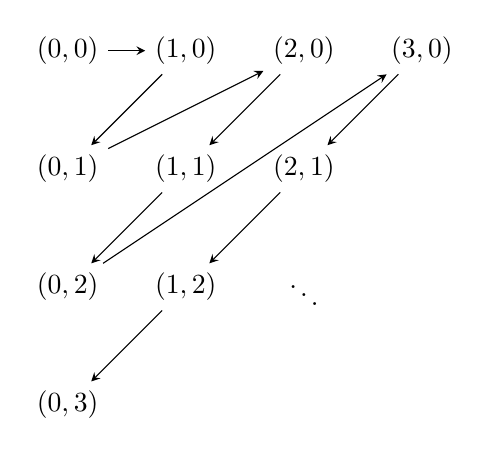
\begin{tikzpicture}[>=stealth, node distance=1.5cm]
        \node (00) {$(0, 0)$};
        \node[right of=00] (10) {$(1, 0)$};
        \node[right of=10] (20) {$(2, 0)$};
        \node[right of=20] (30) {$(3, 0)$};

        \node[below of=00] (01) {$(0, 1)$};
        \node[below of=10] (11) {$(1, 1)$};
        \node[below of=20] (21) {$(2, 1)$};
        \node[below of=01] (02) {$(0, 2)$};
        \node[below of=11] (12) {$(1, 2)$};
        \node[below of=02] (03) {$(0, 3)$};

        \node[right of=12] {$\ddots$};

        % Draw the ordering
        \draw[->] (00) edge (10) (10) edge (01) (01) edge (20) (20) edge
        (11) (11) edge (02) (02) edge (30) (30) edge (21) (21) edge (12)
        (12) edge (03);
    \end{tikzpicture}
    \caption{The Cantor pairing function}\label{fig:cross-ordering}
\end{figure}

and defined by
\[f(n, m) = \frac{1}{2}(n + m)(n + m + 1) + m\]
with inverse
\[f^{-1}(z) = \begin{cases}y = z - \frac{w^2 + w}{2}\\ x = w - y\end{cases}\]
where $\displaystyle w = \floor*{\frac{\sqrt{8z + 1} - 1}{2}}$. The proof that $f$ is a bijection
is quite tedious, so I prefer the proof given above.

\section{}
\begin{quote}
    Watch the following TED-ed talk about the Hilbert's paradox of the Grand
    Hotel.
    \begin{center}
        \url{https://www.youtube.com/watch?v=Uj3_KqkI9Zo}
    \end{center}
    Then show that the night manager could have accomplished the same result
    for the infinitely many coaches with infinitely many seats problem using
    the \textit{prime factorization method} rather than the \textit{prime
        powers method}.
\end{quote}
\end{document}
